% CEEHRC 2026 poster, portrait: 34 in wide x 44 in high (ANSI E), inside the
% conference's 44 x 44 in limit.
%
% Three rows. Row 1: the three text boxes across. Row 2: the schematic workflow
% at full width. Row 3: downstream utility and the references | the challenge
% section. The row heights are set by the tallest column; the log lines
% "POSTER: ... needs" say how much each column needs.
% Build: bash build.sh
\documentclass{article}
\usepackage[paperwidth=34in, paperheight=44in,
            left=0.8in, right=0.8in, top=4.45in, bottom=0.7in]{geometry}
\newcommand{\bodysize}{\fontsize{28}{36}\selectfont}
\newcommand{\capsize}{\fontsize{24}{31}\selectfont}
\newcommand{\smallsize}{\fontsize{19}{24}\selectfont}
\newcommand{\headsize}{\fontsize{44}{53}\selectfont}
\newcommand{\boxtitlesize}{\fontsize{34}{41}\selectfont}
% Input by poster_landscape.tex: packages, colours, the panel and box styles,
% and every sentence on the poster. The layout file sets its page with geometry
% and its type scale (\bodysize, \capsize, \smallsize, \headsize), then inputs
% this file. make_html.py reads the sentences too.
\usepackage[T1]{fontenc}
\usepackage{lmodern}                 % scalable math at poster sizes
\usepackage[default]{opensans}
\usepackage{amsmath,xcolor,graphicx,tikz,qrcode,enumitem}
\usetikzlibrary{calc}
\pagestyle{empty}
\setlength{\parindent}{0pt}
\setlength{\parskip}{0pt}

\definecolor{sfured}{HTML}{A6192E}
\definecolor{ink}{HTML}{1B2A32}
\definecolor{muted}{HTML}{5E6E78}
% The pastel palette. SFU red is only the header block. Headings are deep slate;
% the slate-blue accent and the cool fill carry the boxes and rules. The figures
% use the same family (make_eic_panels.py, split_ga.py): coral for CANDI only,
% mustard for the baseline, dusty blue for signal, sage and lavender for the rest.
\definecolor{heading}{HTML}{2E4A62}
\definecolor{accent}{HTML}{A9BFD3}
\definecolor{panel}{HTML}{F3F6F9}
\definecolor{rule}{HTML}{D9E1E8}

\newcommand{\sectionbar}[1]{%
  {\headsize\bfseries\color{heading}#1\par}\vspace{0.08in}%
  {\color{accent}\rule{\linewidth}{5pt}}\par\vspace{0.3in}}

% One panel: its graphic, then its one- or two-sentence caption.
\newcommand{\panel}[3]{% #1 width  #2 graphic  #3 caption
  \begin{minipage}[t]{#1}
    \vspace{0pt}
    \includegraphics[width=\linewidth]{#2}\par\vspace{0.2in}
    {\capsize\color{ink}\raggedright#3\par}
  \end{minipage}}

\setlist[itemize]{leftmargin=1.0em, itemsep=0.15in, topsep=0.05in,
                  label={\color{accent}\textbullet}}

% ------------------------------------------------------------------ the words --
\newcommand{\PosterTitle}{Self-supervised confidence-aware denoising imputation of genomic data}
\newcommand{\PosterAuthors}{Mehdi Foroozandeh, Abdul Rahman Diab, and Maxwell Libbrecht}
\newcommand{\PosterAffil}{Simon Fraser University, Department of Computing Science}
\newcommand{\PosterURL}{https://mehdiforoozandeh.github.io/CANDI/}

% The problem statement follows the introduction of the MLCB 2026 submission
% (SSL/EpiDenoise/candi-mlcb-2026/main.pdf). Of the four downstream applications
% (make_intro_panels.py), three are ones ChromImpute [1] demonstrates with imputed
% data; the fourth is what CANDI's predicted intervals allow [3].
\newcommand{\HeadProblem}{The problem}
\newcommand{\TxtProblem}{%
\begin{itemize}
  \item Epigenomic data form a 3-D tensor: tens to hundreds of assays
        $\times$ thousands of cell types $\times$ genomic positions.
  \item Profiling every assay in every cell type costs too much, so most
        experiments are missing.
  \item Imputation predicts these missing experiments~[1,2].
  \item Imputed data are often cleaner than observed data, so imputation also
        denoises performed experiments~[1].
  \item Experimental covariates matter: in the ENCODE Imputation Challenge, a
        train--test shift let a simple average-activity baseline beat most
        entrants~[2].
\end{itemize}}

\newcommand{\HeadUses}{Downstream applications}
\newcommand{\TxtUseStates}{Annotate chromatin states in every cell type~[1].}
\newcommand{\TxtUseGwas}{Link disease-associated variants to relevant cell types~[1].}
\newcommand{\TxtUseExpr}{Predict gene expression from marks around each gene~[1,3].}
\newcommand{\TxtUseConf}{Keep confident predictions; set aside uncertain ones~[3].}

\newcommand{\HeadStrip}{CANDI schematic workflow}
\newcommand{\CapStrip}{%
\textbf{Top:} for each 30\,kb locus, CANDI takes observed read counts with the
ChIP-seq control, four covariates per assay and the DNA sequence; grey assays were
never measured, yellow ones are masked. \textbf{Bottom:} each output is a
probability distribution, here a mean and 95\% interval per assay; window by
window, they fill every missing thread of the tensor.}

\newcommand{\HeadEIC}{CANDI fixes the train-test covariate shift in the ENCODE Imputation Challenge}
\newcommand{\CapA}{%
\textbf{A}\enspace Genome-wide Pearson $r$ of CANDI against each of the 51
blind-test experiments (points), by assay.}
\newcommand{\CapB}{%
\textbf{B}\enspace Skill as submitted (filled) and after the same correction
for every entry (open); 1 is the baseline. CANDI is first both ways.}
\newcommand{\CapC}{%
\textbf{C}\enspace Eight of the nine measures relative to the baseline, median
over 51 experiments. CANDI is first on three and
top 8 on the rest.}

\newcommand{\HeadUtility}{Downstream utility of CANDI}
\newcommand{\CapD}{%
\textbf{D}\enspace Confidence calibration for DNase-seq (DND-41): predicted
confidence level against the fraction of observed data within that interval.}
\newcommand{\CapE}{%
\textbf{E}\enspace Gene expression prediction as input assays are removed.
Denoised+Imputed and Latent settings are robust to input sparsity.}

\newcommand{\TxtRefs}{%
[1]~Ernst J, Kellis M. Large-scale imputation of epigenomic datasets for systematic
annotation of diverse human tissues. \textit{Nat Biotechnol} 33:364--376 (2015).\par
[2]~Schreiber J, Boix C, \textit{et al.} The ENCODE Imputation Challenge: a critical
assessment of methods for cross-cell type imputation of epigenomic profiles.
\textit{Genome Biol} 24:79 (2023).\par
[3]~Foroozandeh M, Diab AR, Libbrecht M. CANDI: self-supervised, confidence-aware
denoising imputation of genomic data. \textit{bioRxiv} 2025.01.23.634626 (2025).\par
Panels A--C: blind-test scoring from the Libbrecht lab's EIC reproduction;
\emph{baseline} is the challenge's average-activity track. CANDI's output layer is
fitted on training experiments only; the correction in B is fitted on chr22 of each
blind-test experiment and scored on the other 22 chromosomes.}

% \Column{name}{width}{height}{content}: a column of fixed height, top-aligned, so
% \vfill inside it spreads its blocks to the row's height. The build log gets the
% height the content needs ("POSTER: ... needs"), which is how rows are balanced.
\newsavebox\PosterCol
\newcommand{\Column}[4]{%
  \sbox\PosterCol{\begin{minipage}[t]{#2}\vspace{0pt}#4\end{minipage}}%
  \typeout{POSTER: #1 needs \the\dimexpr\ht\PosterCol+\dp\PosterCol\relax\space of #3}%
  \begin{minipage}[t][#3][t]{#2}\vspace{0pt}#4\end{minipage}}


\newcommand{\BoxW}{10.2in}
\newcommand{\LeftW}{12.2in}
\newcommand{\RightW}{19.4in}
\newcommand{\RowOne}{4.9in}
\newcommand{\RowTwo}{16.85in}
\newcommand{\RowThree}{16.0in}

\begin{document}
% ============================================================ header ==========
\begin{tikzpicture}[remember picture, overlay]
  \coordinate (nw) at (current page.north west);
  \coordinate (ne) at (current page.north east);
  \fill[sfured] ($(nw)+(0,-0.6in)$) rectangle ($(nw)+(7.0in,-3.95in)$);
  \node[anchor=south east, inner sep=0pt, text=white]
    at ($(nw)+(6.7in,-3.8in)$) {\fontsize{150}{150}\selectfont SFU};
  \node[anchor=north west, inner sep=0pt, text=ink]
    at ($(nw)+(7.7in,-0.62in)$) {\resizebox{22.0in}{!}{\bfseries
      \begin{tabular}{@{}l@{}}Self-supervised confidence-aware denoising\\
      imputation of genomic data\end{tabular}}};
  \node[anchor=south west, inner sep=0pt, text=ink]
    at ($(nw)+(7.7in,-3.8in)$) {\fontsize{50}{58}\selectfont\PosterAuthors};
  \node[anchor=north east, inner sep=0pt] at ($(ne)+(-0.8in,-0.6in)$)
    {\qrcode[height=2.9in]{\PosterURL}};
  \node[anchor=north east, inner sep=0pt, text=muted] at ($(ne)+(-0.8in,-3.62in)$)
    {\fontsize{17}{20}\selectfont mehdiforoozandeh.github.io/CANDI};
\end{tikzpicture}%
% ============================================================ row 1 ===========
\Column{row 1 problem}{\BoxW}{\RowOne}{%
  \begin{tcolorbox}[textbox, height=\RowOne]\boxtitle{The problem}\TxtProblem\end{tcolorbox}}\hfill
\Column{row 1 candi}{\BoxW}{\RowOne}{%
  \begin{tcolorbox}[textbox, height=\RowOne]\boxtitle{CANDI}\TxtCandi\end{tcolorbox}}\hfill
\Column{row 1 findings}{\BoxW}{\RowOne}{%
  \begin{tcolorbox}[textbox, height=\RowOne]\boxtitle{Key findings}\TxtFindings\end{tcolorbox}}

\vspace{0.5in}
% ============================================================ row 2 ===========
\Column{row 2}{\linewidth}{\RowTwo}{%
  \sectionbar{\HeadStrip}
  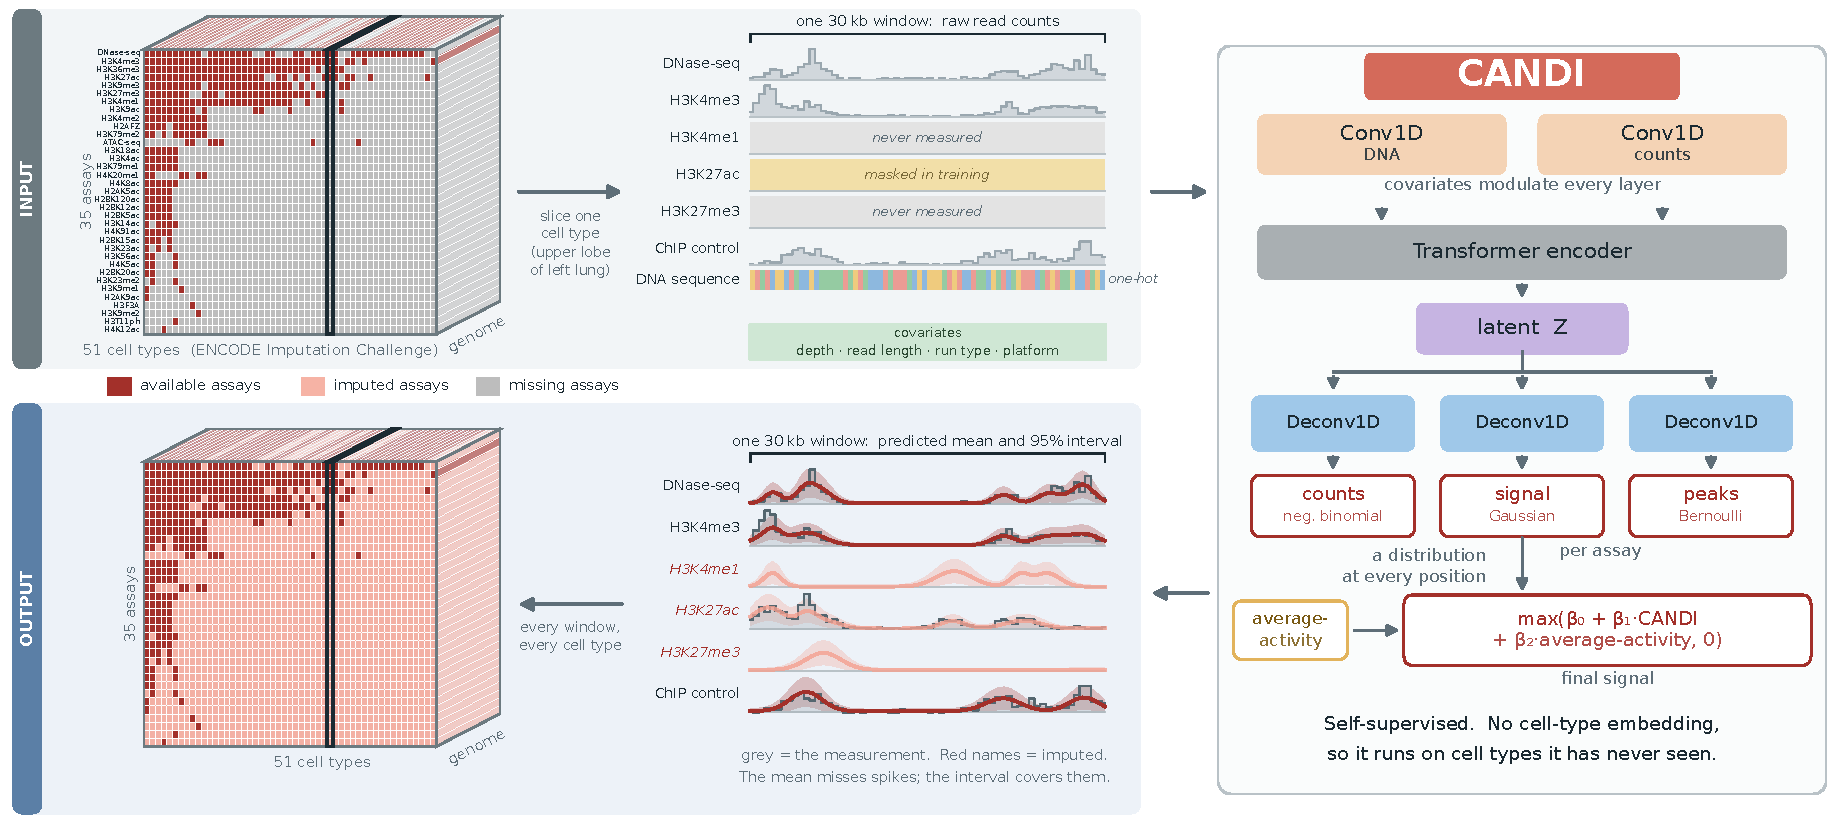
\includegraphics[width=\linewidth]{panels/ga_strip.pdf}\par\vspace{0.25in}
  {\capsize\color{ink}\CapStrip\par}}

\vspace{0.5in}
% ============================================================ row 3 ===========
\Column{row 3 left}{\LeftW}{\RowThree}{%
  \sectionbar{\HeadUtility}
  % Stacked, each caption beside its panel: the panels get more width than
  % they would side by side.
  \begin{minipage}[c]{6.6in}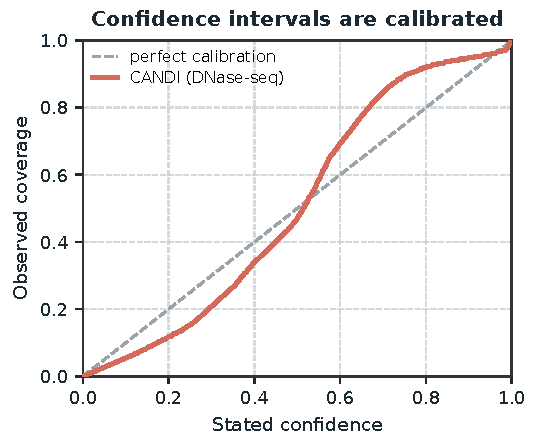
\includegraphics[width=\linewidth]{panels/ga_A.pdf}\end{minipage}\hfill
  \begin{minipage}[c]{5.2in}{\capsize\color{ink}\raggedright\CapA\par}\end{minipage}\par\vspace{0.4in}
  \begin{minipage}[c]{6.6in}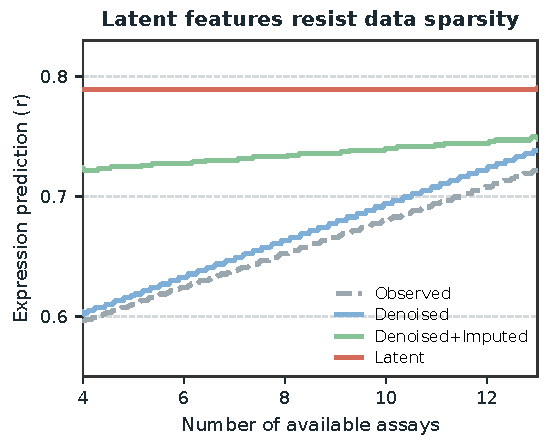
\includegraphics[width=\linewidth]{panels/ga_B.pdf}\end{minipage}\hfill
  \begin{minipage}[c]{5.2in}{\capsize\color{ink}\raggedright\CapB\par}\end{minipage}\par
  \vfill
  {\color{rule}\rule{\linewidth}{3pt}}\par\vspace{0.25in}
  {\smallsize\color{muted}\TxtRefs\par}}\hfill
\Column{row 3 right}{\RightW}{\RowThree}{%
  \sectionbar{\HeadEIC}
  \panel{7.2in}{panels/eic_leaderboard_portrait.pdf}{\CapC}\hfill
  \begin{minipage}[t]{11.6in}\vspace{0pt}
    {\bodysize\color{ink}\TxtEIC\par}\vspace{0.35in}
    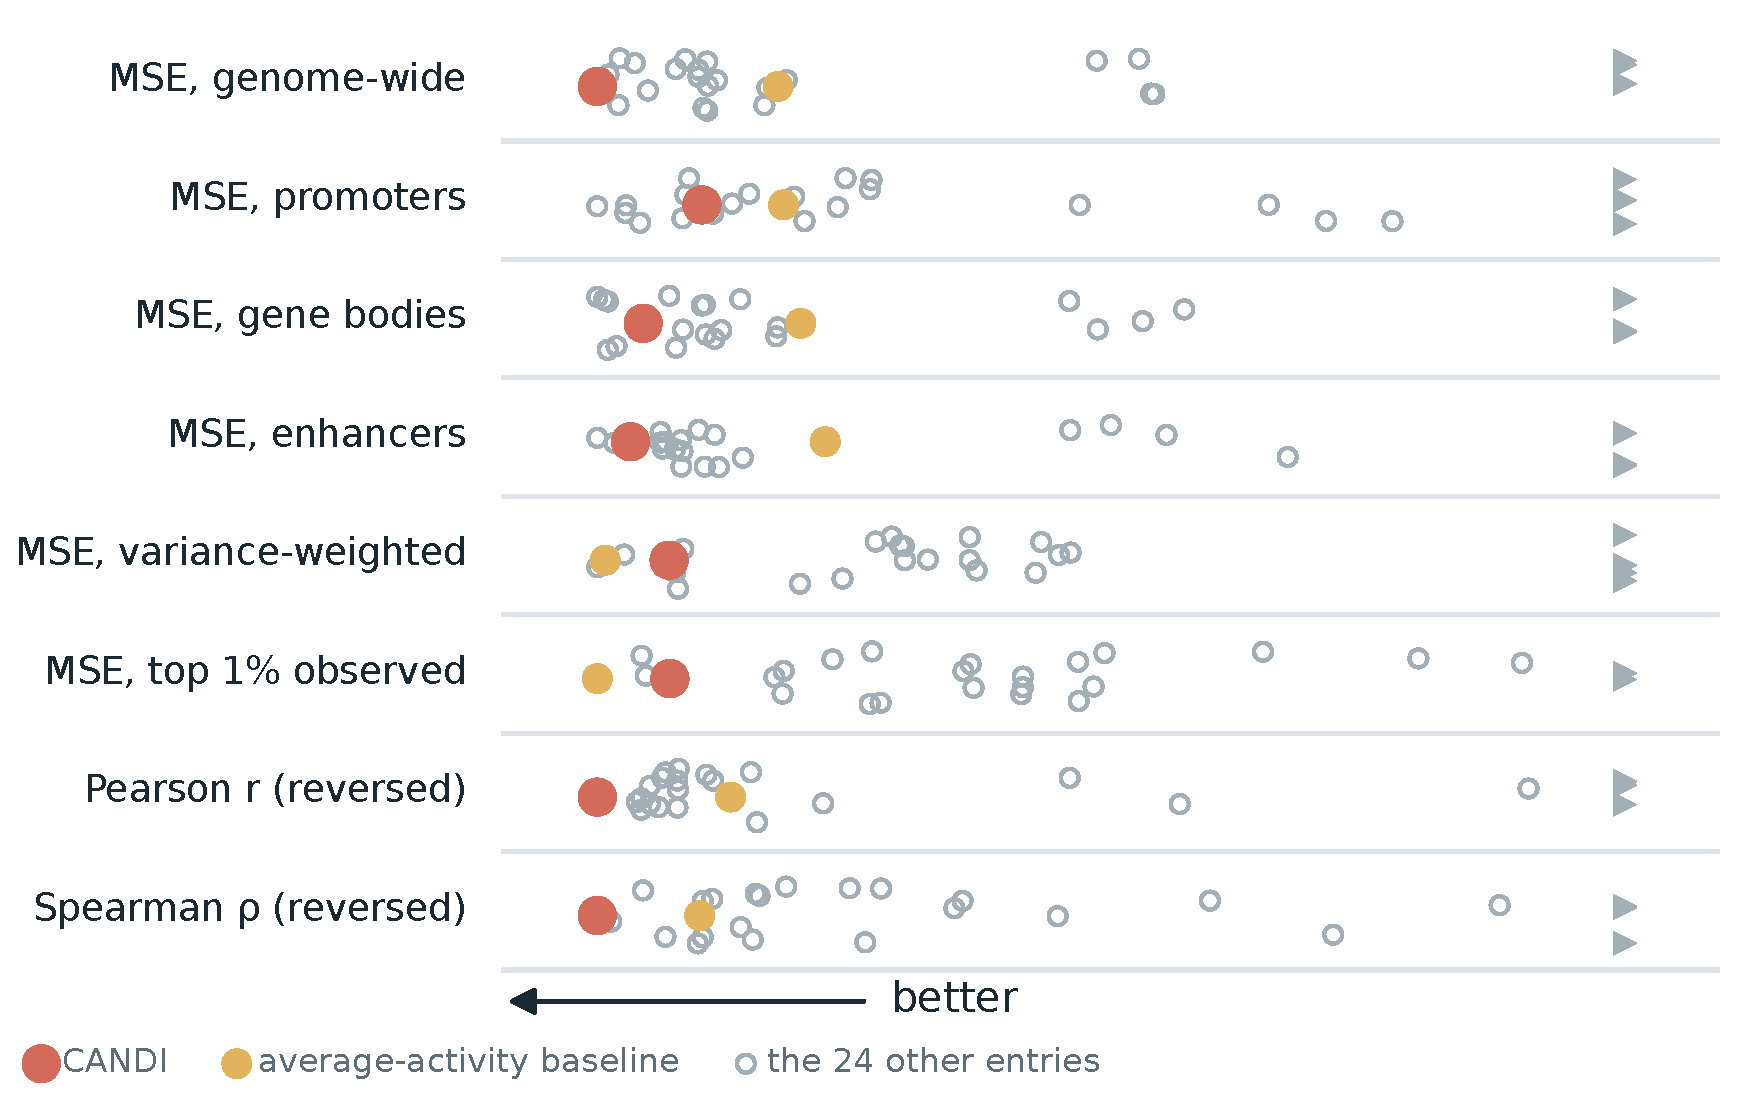
\includegraphics[width=\linewidth]{panels/eic_measures_portrait.pdf}\par\vspace{0.2in}
    {\capsize\color{ink}\CapD\par}
  \end{minipage}}
\end{document}
